\subsection{Position Vector in Polar Co-ordinates}

\begin{definition}
	In polar co-ordinates, {\bf the position vector} i.e. the position of a particle is simply
	$$\underline{r} = r\ \underline{e_{r}}$$
\end{definition}
\vspace{4px}
\begin{mycenter}
	\tikzset{every picture/.style={line width=0.75pt}} %set default line width to 0.75pt        

	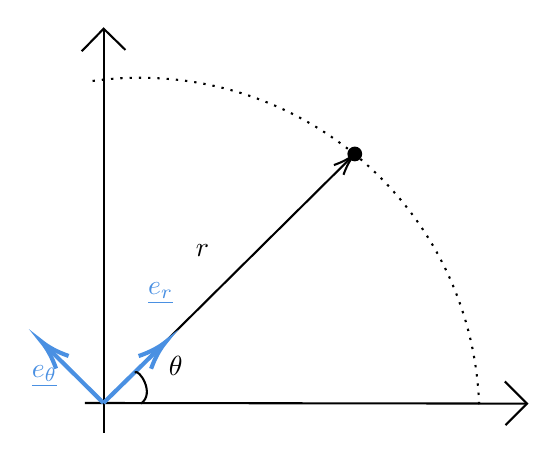
\begin{tikzpicture}[x=0.75pt,y=0.75pt,yscale=-1,xscale=1]
		%uncomment if require: \path (0,402); %set diagram left start at 0, and has height of 402

		%Straight Lines [id:da4134121928340384] 
		\draw    (251.1,37.68) -- (251.1,232.3) ;
		%Straight Lines [id:da5926046353448922] 
		\draw    (242,218) -- (455.1,218.3) ;
		%Straight Lines [id:da5096706615516877] 
		\draw    (251,218) -- (370.68,99.42) ;
		\draw [shift={(372.1,98.02)}, rotate = 135.27] [color={rgb, 255:red, 0; green, 0; blue, 0 }  ][line width=0.75]    (10.93,-3.29) .. controls (6.95,-1.4) and (3.31,-0.3) .. (0,0) .. controls (3.31,0.3) and (6.95,1.4) .. (10.93,3.29)   ;
		%Shape: Circle [id:dp7250045716603137] 
		\draw  [fill={rgb, 255:red, 0; green, 0; blue, 0 }  ,fill opacity=1 ] (369.05,98.02) .. controls (369.05,96.33) and (370.42,94.97) .. (372.1,94.97) .. controls (373.78,94.97) and (375.15,96.33) .. (375.15,98.02) .. controls (375.15,99.7) and (373.78,101.07) .. (372.1,101.07) .. controls (370.42,101.07) and (369.05,99.7) .. (369.05,98.02) -- cycle ;
		%Straight Lines [id:da38254164085879216] 
		\draw [color={rgb, 255:red, 74; green, 144; blue, 226 }  ,draw opacity=1 ][line width=1.5]    (251,218) -- (278.96,190.6) ;
		\draw [shift={(281.1,188.5)}, rotate = 135.58] [color={rgb, 255:red, 74; green, 144; blue, 226 }  ,draw opacity=1 ][line width=1.5]    (14.21,-4.28) .. controls (9.04,-1.82) and (4.3,-0.39) .. (0,0) .. controls (4.3,0.39) and (9.04,1.82) .. (14.21,4.28)   ;
		%Straight Lines [id:da36292628024938856] 
		\draw [color={rgb, 255:red, 74; green, 144; blue, 226 }  ,draw opacity=1 ][line width=1.5]    (251,218) -- (223.23,190.49) ;
		\draw [shift={(221.1,188.38)}, rotate = 44.73] [color={rgb, 255:red, 74; green, 144; blue, 226 }  ,draw opacity=1 ][line width=1.5]    (14.21,-4.28) .. controls (9.04,-1.82) and (4.3,-0.39) .. (0,0) .. controls (4.3,0.39) and (9.04,1.82) .. (14.21,4.28)   ;
		%Curve Lines [id:da4414328655497084] 
		\draw    (266.05,203.25) .. controls (268.1,201.3) and (276.1,213.3) .. (269.1,218.3) ;
		%Shape: Right Angle [id:dp2584901282247881] 
		\draw   (240.54,48.53) -- (251.1,37.68) -- (261.61,47.91) ;
		%Shape: Right Angle [id:dp7209517007920886] 
		\draw   (444.39,207.61) -- (455.1,218.3) -- (444.74,228.68) ;
		%Shape: Arc [id:dp1759431846665106] 
		\draw  [draw opacity=0][dash pattern={on 0.84pt off 2.51pt}] (245.77,62.86) .. controls (253.2,61.83) and (260.79,61.3) .. (268.5,61.3) .. controls (357.9,61.3) and (430.55,132.88) .. (432.08,221.77) -- (268.5,224.62) -- cycle ; \draw  [dash pattern={on 0.84pt off 2.51pt}] (245.77,62.86) .. controls (253.2,61.83) and (260.79,61.3) .. (268.5,61.3) .. controls (357.9,61.3) and (430.55,132.88) .. (432.08,221.77) ;

		% Text Node
		\draw (294,140) node [anchor=north west][inner sep=0.75pt]   [align=left] {$\displaystyle r$};
		% Text Node
		\draw (271,158.48) node [anchor=north west][inner sep=0.75pt]  [color={rgb, 255:red, 74; green, 144; blue, 226 }  ,opacity=1 ] [align=left] {$\displaystyle \underline{e_{r}}$};
		% Text Node
		\draw (215,198.48) node [anchor=north west][inner sep=0.75pt]  [color={rgb, 255:red, 74; green, 144; blue, 226 }  ,opacity=1 ] [align=left] {$\displaystyle \underline{e_{\theta }}$};
		% Text Node
		\draw (281,194) node [anchor=north west][inner sep=0.75pt]   [align=left] {$\displaystyle \theta $};


	\end{tikzpicture}
\end{mycenter}
